\section{Einführung zum Minicase}

Die Familie Meier wohnt in einem dreistöckigen Haus im zweiten Stockwerk. Insgesamt teilen 6 Wohnungen das Haus auf. Eine fortschrittliche Familie aus dem Mittelstand mit bester Reputation.
Bei der Familie Meier wird die IT-Infrastruktur von Onkel Smirnow betreut, welcher von Zeit zu Zeit mit Cracks und anderen Tools das Leben der Familie Meier vereinfacht.
Für diese Familie sollte einen Massnahmenplan für allfällige Risiken gemäss der Aufgabenstellung "Fallstudie: Die Heim PC Lösung" erstellt werden. Für die Eintrittswahrscheinlichkeit und der potenzielle Schaden (Schadensausmass) der Ereignisse wird eine Skala von 1 (sehr kleine(r) Wahrscheinlichkeit/Schaden) bis 4 (sehr grosse(r) Wahrscheinlichkeit/Schaden) verwendet.



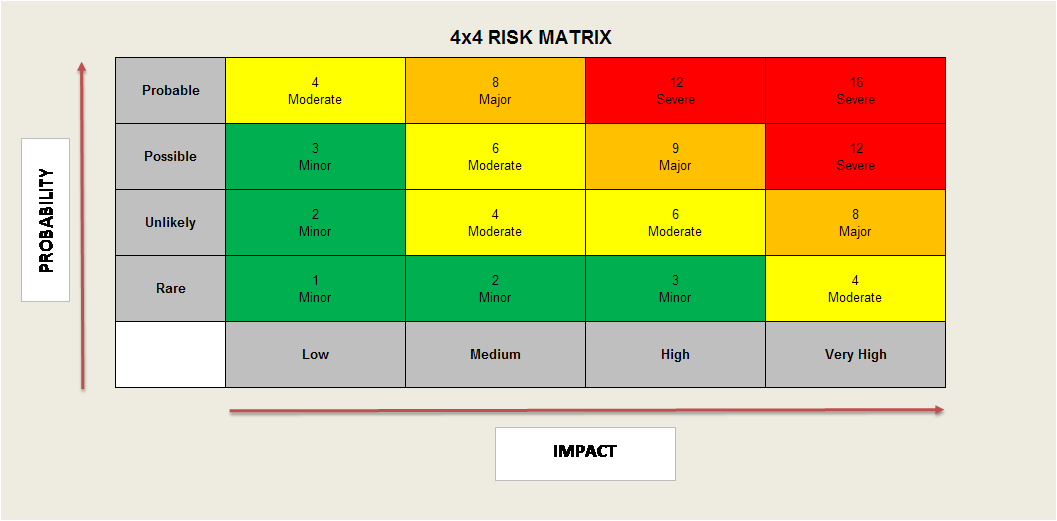
\includegraphics[width=\textwidth]{Risikomatrix}
